\documentclass{report}
\usepackage{fullpage}
\usepackage{graphicx}
\usepackage{array}
\usepackage{float}

\renewcommand{\baselinestretch}{2}
% Redefine the title page
% Redefine the title page
\makeatletter
\renewcommand{\maketitle}{
    \begin{titlepage}
        \centering
        \vspace*{2cm}

        {\Huge \bfseries \@title \par}
        \vspace{1.5cm}
        {\Huge \@author \par}
        
        { Entry Number: 2024AIM1011 \par}
        \vspace{0 cm}
        {Course Code: CS506 \par}
        {\Large Department of Computer Science and Engineering \par}
        \vspace{2cm}
        
        {\Large System Specifications \par}
        \begin{center}
            \begin{tabular}{rl}
                &Processor:  AMD Ryzen 7 3750H \\
                &RAM:  16 GB \\
                &OS: Windows 11 \\
            \end{tabular}
        \end{center}
        
        \vfill
    \end{titlepage}
}
\makeatother

\author{Yash Narnaware}
\title{Sorting Algorithms Analysis}
\begin{document}




\maketitle

\renewcommand{\arraystretch}{0.6}


\setlength{\tabcolsep}{2pt}

\chapter{Sorting Algorithms}


\section{Bubble Sort}
The time complexity of Bubble sort is $O(n)^{2}$ because we have 2 nested for loops (can be while loops also) in its algorithm. Best case is when array is already sorted in that case time complexity becomes $O(n)$ which wee achieve by keeping track of if swapping is happend in that iteration. And worst case is when array is revese sorted.
\section{Selection Sort}
The time complexity of selection sort in best worst and average case is $O(n)^{2}$ because it has 2 nested loops one for choosing minimum and 1 for traversing through array.
\section{Merge Sort}
The time complexity for merge sort is $O(n\log{n})$ in best worst and average cases because in any case we have to divide array in half sizes which takes $O(\log{n})$ time and merging the sorted arrays take $O(n)$ time. So we are dividing array in half till they become sorted(singleton array) and then combine the sorted arrays which altogether takes $O(n\log{n})$ time.
\section{Insertion Sort}
The time complexity of insertion sort is $O(n^2)$ in worst and average case and is $O(n)$ in best case. The best cae is when array is already sorted in this case we don't need to find the correct place for current element in preceeding array. The worst case occures when array is rverse sorted in this case we have go to the start of preceeding array to place the current element.
\section{Quick Sort}

The time complexity of quick sort in best and average case is $O(n\log{n})$ and in worst case is $O(n^2)$.Dividing based on pivot takes $O(n)$ time and passing the divided arrays to quick sort again takes $O(\log{n})$ time so altogether time complexity becomes $O(n\log{n})$. The best case occurs when we select array median as a pivot for partitioning and worst case is when we select the pivot such that array gets divided into 1 and N-1 elements. 

\chapter{Comparing Sorting Algorithms}

I have taken arrays of different sizes and different conditions like sorted,uunsorted ,reverse sorted etc. and plotted graphs of how different sorting algorithms behave on them.

\subsection{How sorting algorithms behave to diffrent array sizes?}

Data in table format - 

\begin{table}[H]
\centering
\begin{tabular}{|c|c|c|c|c|c|}
\hline
\textbf{Size} & \textbf{Bubble Sort} & \textbf{Insertion Sort} & \textbf{Selection Sort} & \textbf{Merge Sort} & \textbf{Quick Sort} \\ \hline
10 & 0 & 0 & 0 & 0 & 0 \\ \hline
100 & 0.00003 & 0.00001 & 0.00002 & 0.00001 & 0.00001 \\ \hline
200 & 0.00009 & 0.00003 & 0.00006 & 0.00002 & 0.00002 \\ \hline
400 & 0.00036 & 0.00012 & 0.00022 & 0.00005 & 0.00004 \\ \hline
800 & 0.00127 & 0.00045 & 0.00085 & 0.0001 & 0.00007 \\ \hline
1600 & 0.0048 & 0.00172 & 0.00327 & 0.00021 & 0.00015 \\ \hline
3200 & 0.01883 & 0.00687 & 0.01282 & 0.00046 & 0.00034 \\ \hline
6400 & 0.07035 & 0.02548 & 0.0349 & 0.00075 & 0.00053 \\ \hline
12800 & 0.2383 & 0.09995 & 0.15588 & 0.00161 & 0.00109 \\ \hline
25600 & 1.38234 & 0.47288 & 0.68966 & 0.00434 & 0.00309 \\ \hline
\end{tabular}
\caption{Sorting Algorithms on different size arrays}
\end{table}

Data in graph format - 


\begin{figure}[H]
\centering
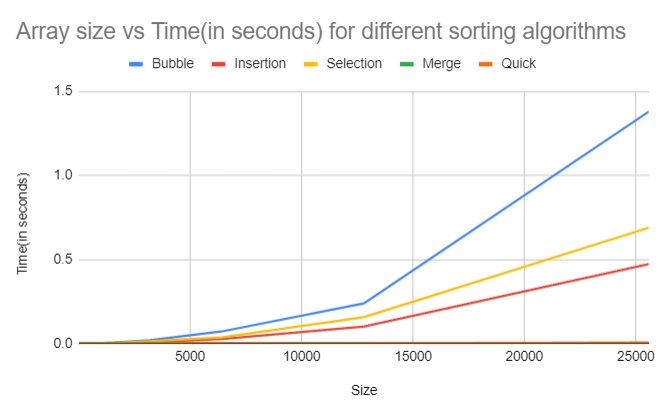
\includegraphics[scale=0.8]{sizevstime.png}

\end{figure}


\subsection{Number of swaps for different array size}

Data in table format -

\begin{table}[H]
\centering
\begin{tabular}{|c|c|c|c|c|}
\hline
\textbf{Array Size} & \textbf{Bubble Sort} & \textbf{Insertion Sort} & \textbf{Selection Sort} & \textbf{Quick Sort} \\ \hline
10 & 37 & 27 & 7 & 10 \\ \hline
100 & 2675 & 2575 & 93 & 158 \\ \hline
200 & 10035 & 9834 & 195 & 377 \\ \hline
400 & 41999 & 41590 & 393 & 857 \\ \hline
800 & 164822 & 163991 & 793 & 1839 \\ \hline
1600 & 640571 & 638857 & 1597 & 4017 \\ \hline
3200 & 2558263 & 2554546 & 3192 & 8878 \\ \hline
6400 & 10336066 & 10327571 & 6389 & 19338 \\ \hline
12800 & 41184565 & 41163493 & 12789 & 41337 \\ \hline
25600 & 161983948 & 161925779 & 25592 & 89208 \\ \hline
\end{tabular}
\caption{Number of swaps for different sorting algorithms on different sized arrays}
\end{table}


Data in graph format - 

\begin{figure}[H]
\centering
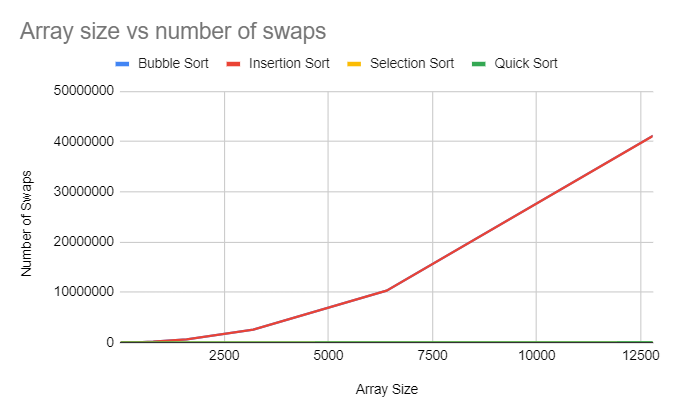
\includegraphics[scale=0.8]{numofswaps.png}
\end{figure}


\subsection{Testing sorting algorithms on already sorted arrays}

\begin{table}[H]
\centering
\begin{tabular}{|c|c|c|c|c|c|}
\hline
\textbf{Array Size} & \textbf{Bubble Sort} & \textbf{Insertion Sort} & \textbf{Selection Sort} & \textbf{Merge Sort} & \textbf{Quick Sort} \\ \hline
10 & 0 & 0 & 0 & 0 & 0 \\ \hline
100 & 0.00001 & 0 & 0.00001 & 0.00001 & 0.00002 \\ \hline
200 & 0.00005 & 0 & 0.00005 & 0.00001 & 0.00004 \\ \hline
400 & 0.0002 & 0 & 0.0002 & 0.00003 & 0.00015 \\ \hline
800 & 0.00079 & 0 & 0.00079 & 0.00005 & 0.00059 \\ \hline
1600 & 0.00309 & 0.00001 & 0.00309 & 0.00012 & 0.00212 \\ \hline
3200 & 0.0121 & 0.00001 & 0.01121 & 0.00019 & 0.00475 \\ \hline
6400 & 0.02746 & 0.00002 & 0.04488 & 0.00054 & 0.02599 \\ \hline
12800 & 0.14739 & 0.00006 & 0.12168 & 0.00087 & 0.07607 \\ \hline
25600 & 0.59978 & 0.00007 & 0.50619 & 0.0018 & 0.27262 \\ \hline
\end{tabular}
\caption{Time taken by Sorting Algorithms on different sized sorted arrays}
\end{table}


Data in graph format - 

\begin{figure}[H]
\centering
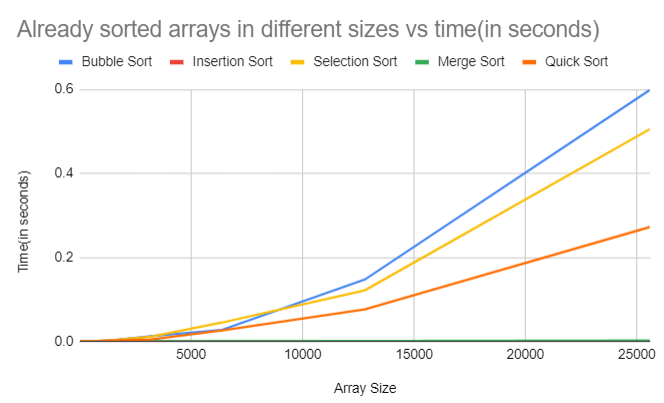
\includegraphics[scale=0.8]{sortedarray.png}
\end{figure}



\subsection{Testing sorting algorithms on arrays in reverse sorted order}

Data in graph format - 




\begin{table}[H]
\centering
\begin{tabular}{|c|c|c|c|c|c|}
\hline
\textbf{Array Size} & \textbf{Bubble Sort} & \textbf{Insertion Sort} & \textbf{Selection Sort} & \textbf{Merge Sort} & \textbf{Quick Sort} \\ \hline
10 & 0 & 0 & 0 & 0 & 0 \\ \hline
100 & 0.00002 & 0.00001 & 0.00003 & 0.00001 & 0.00001 \\ \hline
200 & 0.00007 & 0.00004 & 0.00004 & 0.00001 & 0.00003 \\ \hline
400 & 0.00028 & 0.00015 & 0.00013 & 0.00002 & 0.0001 \\ \hline
800 & 0.0011 & 0.00057 & 0.0005 & 0.00004 & 0.00034 \\ \hline
1600 & 0.0042 & 0.00303 & 0.00199 & 0.00009 & 0.00137 \\ \hline
3200 & 0.01695 & 0.00928 & 0.00769 & 0.00019 & 0.00518 \\ \hline
6400 & 0.06711 & 0.037 & 0.03188 & 0.00041 & 0.02078 \\ \hline
12800 & 0.31812 & 0.18226 & 0.14792 & 0.00091 & 0.10011 \\ \hline
25600 & 1.15921 & 0.78429 & 0.76152 & 0.00179 & 0.35887 \\ \hline
\end{tabular}
\caption{Time taken by Sorting Algorithms on different sized reverse sorted arrays}
\end{table}

\begin{figure}[H]
\centering
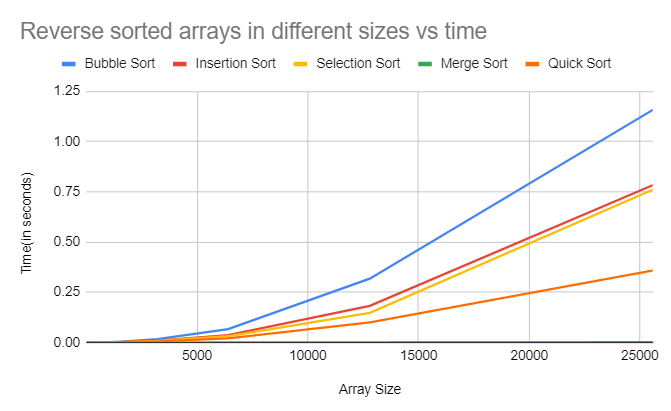
\includegraphics[scale=0.8]{reversesorted.png}

\end{figure}

\end{document}